% Options for packages loaded elsewhere
\PassOptionsToPackage{unicode}{hyperref}
\PassOptionsToPackage{hyphens}{url}
\PassOptionsToPackage{dvipsnames,svgnames*,x11names*}{xcolor}
%
\documentclass[
]{article}
\usepackage{amsmath,amssymb}
\usepackage{lmodern}
\usepackage{ifxetex,ifluatex}
\ifnum 0\ifxetex 1\fi\ifluatex 1\fi=0 % if pdftex
  \usepackage[T1]{fontenc}
  \usepackage[utf8]{inputenc}
  \usepackage{textcomp} % provide euro and other symbols
\else % if luatex or xetex
  \usepackage{unicode-math}
  \defaultfontfeatures{Scale=MatchLowercase}
  \defaultfontfeatures[\rmfamily]{Ligatures=TeX,Scale=1}
\fi
% Use upquote if available, for straight quotes in verbatim environments
\IfFileExists{upquote.sty}{\usepackage{upquote}}{}
\IfFileExists{microtype.sty}{% use microtype if available
  \usepackage[]{microtype}
  \UseMicrotypeSet[protrusion]{basicmath} % disable protrusion for tt fonts
}{}
\makeatletter
\@ifundefined{KOMAClassName}{% if non-KOMA class
  \IfFileExists{parskip.sty}{%
    \usepackage{parskip}
  }{% else
    \setlength{\parindent}{0pt}
    \setlength{\parskip}{6pt plus 2pt minus 1pt}}
}{% if KOMA class
  \KOMAoptions{parskip=half}}
\makeatother
\usepackage{xcolor}
\IfFileExists{xurl.sty}{\usepackage{xurl}}{} % add URL line breaks if available
\IfFileExists{bookmark.sty}{\usepackage{bookmark}}{\usepackage{hyperref}}
\hypersetup{
  pdftitle={Week 2: Glucocorticoid receptor dynamica},
  pdfauthor={Jurrien de Jong en Miguel Botter van Elburg},
  colorlinks=true,
  linkcolor=blue,
  filecolor=Maroon,
  citecolor=Blue,
  urlcolor=Blue,
  pdfcreator={LaTeX via pandoc}}
\urlstyle{same} % disable monospaced font for URLs
\usepackage[margin=1in]{geometry}
\usepackage{color}
\usepackage{fancyvrb}
\newcommand{\VerbBar}{|}
\newcommand{\VERB}{\Verb[commandchars=\\\{\}]}
\DefineVerbatimEnvironment{Highlighting}{Verbatim}{commandchars=\\\{\}}
% Add ',fontsize=\small' for more characters per line
\usepackage{framed}
\definecolor{shadecolor}{RGB}{248,248,248}
\newenvironment{Shaded}{\begin{snugshade}}{\end{snugshade}}
\newcommand{\AlertTok}[1]{\textcolor[rgb]{0.94,0.16,0.16}{#1}}
\newcommand{\AnnotationTok}[1]{\textcolor[rgb]{0.56,0.35,0.01}{\textbf{\textit{#1}}}}
\newcommand{\AttributeTok}[1]{\textcolor[rgb]{0.77,0.63,0.00}{#1}}
\newcommand{\BaseNTok}[1]{\textcolor[rgb]{0.00,0.00,0.81}{#1}}
\newcommand{\BuiltInTok}[1]{#1}
\newcommand{\CharTok}[1]{\textcolor[rgb]{0.31,0.60,0.02}{#1}}
\newcommand{\CommentTok}[1]{\textcolor[rgb]{0.56,0.35,0.01}{\textit{#1}}}
\newcommand{\CommentVarTok}[1]{\textcolor[rgb]{0.56,0.35,0.01}{\textbf{\textit{#1}}}}
\newcommand{\ConstantTok}[1]{\textcolor[rgb]{0.00,0.00,0.00}{#1}}
\newcommand{\ControlFlowTok}[1]{\textcolor[rgb]{0.13,0.29,0.53}{\textbf{#1}}}
\newcommand{\DataTypeTok}[1]{\textcolor[rgb]{0.13,0.29,0.53}{#1}}
\newcommand{\DecValTok}[1]{\textcolor[rgb]{0.00,0.00,0.81}{#1}}
\newcommand{\DocumentationTok}[1]{\textcolor[rgb]{0.56,0.35,0.01}{\textbf{\textit{#1}}}}
\newcommand{\ErrorTok}[1]{\textcolor[rgb]{0.64,0.00,0.00}{\textbf{#1}}}
\newcommand{\ExtensionTok}[1]{#1}
\newcommand{\FloatTok}[1]{\textcolor[rgb]{0.00,0.00,0.81}{#1}}
\newcommand{\FunctionTok}[1]{\textcolor[rgb]{0.00,0.00,0.00}{#1}}
\newcommand{\ImportTok}[1]{#1}
\newcommand{\InformationTok}[1]{\textcolor[rgb]{0.56,0.35,0.01}{\textbf{\textit{#1}}}}
\newcommand{\KeywordTok}[1]{\textcolor[rgb]{0.13,0.29,0.53}{\textbf{#1}}}
\newcommand{\NormalTok}[1]{#1}
\newcommand{\OperatorTok}[1]{\textcolor[rgb]{0.81,0.36,0.00}{\textbf{#1}}}
\newcommand{\OtherTok}[1]{\textcolor[rgb]{0.56,0.35,0.01}{#1}}
\newcommand{\PreprocessorTok}[1]{\textcolor[rgb]{0.56,0.35,0.01}{\textit{#1}}}
\newcommand{\RegionMarkerTok}[1]{#1}
\newcommand{\SpecialCharTok}[1]{\textcolor[rgb]{0.00,0.00,0.00}{#1}}
\newcommand{\SpecialStringTok}[1]{\textcolor[rgb]{0.31,0.60,0.02}{#1}}
\newcommand{\StringTok}[1]{\textcolor[rgb]{0.31,0.60,0.02}{#1}}
\newcommand{\VariableTok}[1]{\textcolor[rgb]{0.00,0.00,0.00}{#1}}
\newcommand{\VerbatimStringTok}[1]{\textcolor[rgb]{0.31,0.60,0.02}{#1}}
\newcommand{\WarningTok}[1]{\textcolor[rgb]{0.56,0.35,0.01}{\textbf{\textit{#1}}}}
\usepackage{graphicx}
\makeatletter
\def\maxwidth{\ifdim\Gin@nat@width>\linewidth\linewidth\else\Gin@nat@width\fi}
\def\maxheight{\ifdim\Gin@nat@height>\textheight\textheight\else\Gin@nat@height\fi}
\makeatother
% Scale images if necessary, so that they will not overflow the page
% margins by default, and it is still possible to overwrite the defaults
% using explicit options in \includegraphics[width, height, ...]{}
\setkeys{Gin}{width=\maxwidth,height=\maxheight,keepaspectratio}
% Set default figure placement to htbp
\makeatletter
\def\fps@figure{htbp}
\makeatother
\setlength{\emergencystretch}{3em} % prevent overfull lines
\providecommand{\tightlist}{%
  \setlength{\itemsep}{0pt}\setlength{\parskip}{0pt}}
\setcounter{secnumdepth}{-\maxdimen} % remove section numbering
\usepackage{longtable}
\usepackage{hyperref}
\ifluatex
  \usepackage{selnolig}  % disable illegal ligatures
\fi
\newlength{\cslhangindent}
\setlength{\cslhangindent}{1.5em}
\newlength{\csllabelwidth}
\setlength{\csllabelwidth}{3em}
\newenvironment{CSLReferences}[2] % #1 hanging-ident, #2 entry spacing
 {% don't indent paragraphs
  \setlength{\parindent}{0pt}
  % turn on hanging indent if param 1 is 1
  \ifodd #1 \everypar{\setlength{\hangindent}{\cslhangindent}}\ignorespaces\fi
  % set entry spacing
  \ifnum #2 > 0
  \setlength{\parskip}{#2\baselineskip}
  \fi
 }%
 {}
\usepackage{calc}
\newcommand{\CSLBlock}[1]{#1\hfill\break}
\newcommand{\CSLLeftMargin}[1]{\parbox[t]{\csllabelwidth}{#1}}
\newcommand{\CSLRightInline}[1]{\parbox[t]{\linewidth - \csllabelwidth}{#1}\break}
\newcommand{\CSLIndent}[1]{\hspace{\cslhangindent}#1}

\title{Week 2: Glucocorticoid receptor dynamica}
\author{Jurrien de Jong en Miguel Botter van Elburg}
\date{2021-05-10}

\begin{document}
\maketitle

\hypertarget{introduction}{%
\section{Introduction}\label{introduction}}

Corticosteroïden zijn chemische stoffen met een structuur die lijkt op
de structuur van hormonen die door de bijnier worden aangemaakt. Deze
bijnierhormonen, zoals bijvoorbeeld cortisol, spelen een rol bij
ontstekingen en de afweer tegen infecties ({``Corticosteroïden --
Werking, Toepassingen, Bijwerkingen - Simpto.nl,''} n.d.).

\hypertarget{goal}{%
\subsection{Goal}\label{goal}}

In dit onderzoek staat het biologisch model van het Corticoide hormoon
centraal. De volgende relevante zaken worden behandelt;

\begin{itemize}
\tightlist
\item
  Welke parameters moeten er geprogrammeerd worden?
\item
  Er moeten internet bronnen gevonden worden waar het biologisch model
  vandaan komt.
\item
  We moeten een biologisch model ontwerpen en we leggen de formule door
  middel van een vertaling uit.
\item
  Achterhalen wat de return waarde van de model functie in R is, daarna
  deze verder toelichten (waarom we deze returnen en niet R zelf).
\end{itemize}

\hypertarget{theory}{%
\subsection{Theory}\label{theory}}

Bij een corticosteroïden behandeling wordt een medicijn (hormoon
corticosteroïd) in een gewricht, peesschede of rond de zenuw gebracht.
De corticosteroïden hebben een ontstekingsremmende werking en geven de
geprikkelde zenuwen rust ({``Corticosteroïden Injectie \textbar{}
OLVG,''} n.d.).

Enkele voorbeelden van corticosteroïden zijn; Predniso(lo)n,
Dexamethason, (Hydro)cortison, Triamcinolon, Betametason, Fluticason
({``Corticosteroiden (Medicinfo.nl),''} n.d.).

De werking van corticosteroïden verschilt. Dit geldt voor sterkte,
toedieningsvorm en mate van bijwerkingen. Het kan voorgeschreven worden
als stootkuur (korte periode een hoge dosering), maar ook langdurig als
onderhoudsbehandeling. In het geval van longpatiënten worden
corticosteroïden gebruikt als ontstekingsremmer en worden ze ingezet bij
allergische reacties op uitwendige prikkels (vb: hooikoorts, eczeem)
({``Corticosteroïden - VND (Nederland-Davos.nl),''} n.d.).

\hypertarget{methods}{%
\section{Methods}\label{methods}}

In dit onderzoek worden de parameters R en m geprogrammeerd van het
model gemodelleerd, omdat deze variabel per tijdseenheid zijn. Desolve
v1.28 is gebruikt voor de visualisatie van de grafieken.

\hypertarget{the-software-model}{%
\subsection{The software model}\label{the-software-model}}

De glucocorticoiden zullen met name meerdere ontstekings geactiveerde
genen uitzetten, die coderen voor cytokines, chemokines, hechtings
moleculen van ontstoken enzymen en receptors (zie Fig 1). Deze genen
zijn aangezet in de luchtwegen door pro-ontstekings transcriptie
factoren, zoals nuclear factor-κB (NF-κB) en activator protein-1 (AP-1),
die normaal gesproken beide worden geactiveerd in de buurt van asthma en
COPD ontstekingen (zie Fig 2).

\begin{Shaded}
\begin{Highlighting}[]
\NormalTok{knitr}\SpecialCharTok{::}\FunctionTok{include\_graphics}\NormalTok{(}\StringTok{\textquotesingle{}Fig1\_week2.png.jpg\textquotesingle{}}\NormalTok{)}
\end{Highlighting}
\end{Shaded}

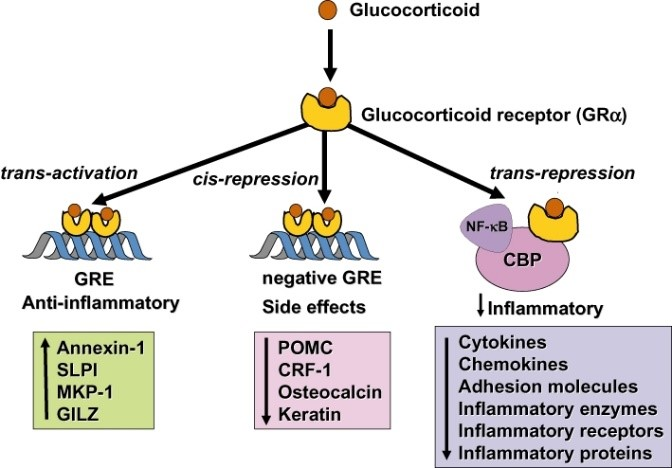
\includegraphics{Fig1_week2.png.jpg}

\begin{Shaded}
\begin{Highlighting}[]
\NormalTok{knitr}\SpecialCharTok{::}\FunctionTok{include\_graphics}\NormalTok{(}\StringTok{\textquotesingle{}Fig2\_week2.png.jpg\textquotesingle{}}\NormalTok{)}
\end{Highlighting}
\end{Shaded}

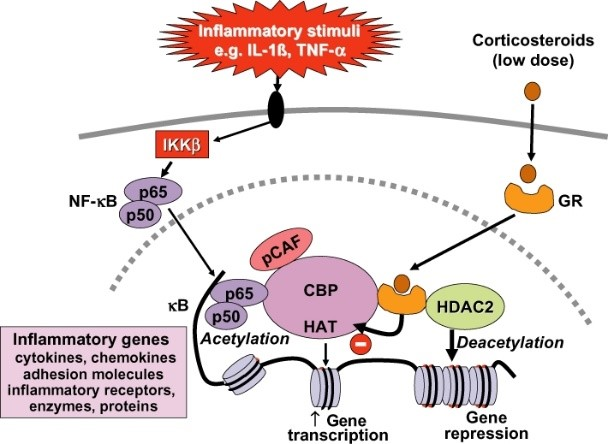
\includegraphics{Fig2_week2.png.jpg}

\hypertarget{model-configuration}{%
\subsection{Model configuration}\label{model-configuration}}

De tijdslengte die gekozen is, is 48 uur ( omdat dit 2 dagen is en zo
een onderzoeksvraag beantwoord ). Verder zijn de parameters en values
die gegeven waren via de opdracht gebruikt omdat dit feitelijke, en goed
onderzochte waardes zijn. Hier in deze tabel een overzicht van de
gebruikte waardes:

\begin{longtable}[l]{l|l|l}
\caption{Parameter Values} \\ \hline
\label{param_table}
$\textbf{Parameter}$             &$\textbf{Value}$& $\textbf{Unit}$              \\ \hline
\endhead
$IC50_Rm$       & 26.2  & $fmol/mg protein$         \\ \hline
$kon$       & 0.00329  & $L/nmol/h$         \\ \hline
$kT$       & 0.63  & $1 / hour$         \\ \hline
$kre$       & 0.57  & $1 / hour$         \\ \hline
$Rf$       & 0.49  & $x$         \\ \hline
$kd_R$       & 0.0572  & $1 / hour$         \\ \hline
$kd_Rm$       & 0.612  & $x$         \\ \hline
$ks_r$       & 3.22  & $x$         \\ \hline
$D$       & 53.40868  & $nmol/L$         \\ \hline
$Rm0$       & 4.74  & $fmol/g liver$         \\ \hline
$R0$       & 267  & $fmol/mg protein$         \\ \hline
$DR$       & 0  & $fmol/mg protein$         \\ \hline
$DR(N)$       & 0  & $fmol/mg protein$         \\ \hline
\end{longtable}

\hypertarget{results}{%
\section{Results}\label{results}}

De vragen die opkomen tijdens het onderzoeken van een biologisch systeem
zal je kunnen beantwoorden aan de hand van een gecreerd model. Hieronder
is de code te zien dat zo'n soort model kan produceren:

\begin{Shaded}
\begin{Highlighting}[]
\CommentTok{\# Change the MPL value from mol/L to nmol/L}
\NormalTok{D }\OtherTok{\textless{}{-}} \DecValTok{20} \SpecialCharTok{*} \DecValTok{1000} \SpecialCharTok{/} \FloatTok{374.471}
\FunctionTok{cat}\NormalTok{(}\StringTok{"D :"}\NormalTok{, D)}
\end{Highlighting}
\end{Shaded}

\begin{verbatim}
## D : 53.40868
\end{verbatim}

\begin{Shaded}
\begin{Highlighting}[]
\CommentTok{\# Parameters to be used in the Glucocorticoid function}
\NormalTok{parameters }\OtherTok{\textless{}{-}} \FunctionTok{c}\NormalTok{(}\AttributeTok{ks\_Rm =} \FloatTok{2.90}\NormalTok{, }\AttributeTok{IC50\_Rm =} \FloatTok{26.2}\NormalTok{, }\AttributeTok{kon =} \FloatTok{0.00329}\NormalTok{,}
                \AttributeTok{kT =} \FloatTok{0.63}\NormalTok{, }\AttributeTok{kre =} \FloatTok{0.57}\NormalTok{, }\AttributeTok{Rf =} \FloatTok{0.49}\NormalTok{, }\AttributeTok{kd\_R =} \FloatTok{0.0572}\NormalTok{,}
                \AttributeTok{kd\_Rm =} \FloatTok{0.612}\NormalTok{, }\AttributeTok{ks\_r =} \FloatTok{3.22}\NormalTok{, D, }\AttributeTok{Rm0 =} \FloatTok{4.74}\NormalTok{,}
                \AttributeTok{DR =} \DecValTok{0}\NormalTok{, }\AttributeTok{DRN =} \DecValTok{0}\NormalTok{)}

\CommentTok{\# this function calculates the derivatives and returns it as a list.}
\NormalTok{Glucocorticoid\_func }\OtherTok{\textless{}{-}} \ControlFlowTok{function}\NormalTok{(t, y, parms) \{}
    \FunctionTok{with}\NormalTok{(}\FunctionTok{as.list}\NormalTok{(}\FunctionTok{c}\NormalTok{(y, parms)),\{}
      
      \CommentTok{\# Dit model bevat 4 afgeleide functies:}
      \CommentTok{\# Afgeleide 1:}
  
\NormalTok{      dmRNAr\_dt }\OtherTok{\textless{}{-}}\NormalTok{ ks\_Rm }\SpecialCharTok{*}\NormalTok{ ( }\DecValTok{1} \SpecialCharTok{{-}}\NormalTok{ (DRN }\SpecialCharTok{/}\NormalTok{ (IC50\_Rm }\SpecialCharTok{+}\NormalTok{ DRN))) }\SpecialCharTok{{-}}\NormalTok{ kd\_Rm }\SpecialCharTok{*}\NormalTok{ mRNAr}
  
      \CommentTok{\# Afgeleide 2:}
  
\NormalTok{      dR\_dt }\OtherTok{\textless{}{-}}\NormalTok{ ks\_r }\SpecialCharTok{*}\NormalTok{ mRNAr }\SpecialCharTok{+}\NormalTok{ Rf }\SpecialCharTok{*}\NormalTok{ kre }\SpecialCharTok{*}\NormalTok{ DRN }\SpecialCharTok{{-}}\NormalTok{ kon }\SpecialCharTok{*}\NormalTok{ D }\SpecialCharTok{*}\NormalTok{ R }\SpecialCharTok{{-}}\NormalTok{ kd\_R }\SpecialCharTok{*}\NormalTok{ R}
      
      \CommentTok{\# Afgeleide 3:}
  
\NormalTok{      dDR\_dt }\OtherTok{\textless{}{-}}\NormalTok{ kon }\SpecialCharTok{*}\NormalTok{ D }\SpecialCharTok{*}\NormalTok{ R }\SpecialCharTok{{-}}\NormalTok{ kT }\SpecialCharTok{*}\NormalTok{ DR}
  
      \CommentTok{\# Afgeleide 4:}
  
\NormalTok{      dDRN\_dt }\OtherTok{\textless{}{-}}\NormalTok{ kT }\SpecialCharTok{*}\NormalTok{ DR }\SpecialCharTok{{-}}\NormalTok{ kre }\SpecialCharTok{*}\NormalTok{ DRN}
      
      \FunctionTok{return}\NormalTok{(}\FunctionTok{list}\NormalTok{(}\FunctionTok{c}\NormalTok{(dmRNAr\_dt, dR\_dt, dDR\_dt, dDRN\_dt)))}
\NormalTok{       \}}
\NormalTok{       )}
\NormalTok{\}}

\CommentTok{\# Set initial values}
\NormalTok{state }\OtherTok{\textless{}{-}} \FunctionTok{c}\NormalTok{(}\AttributeTok{mRNAr =} \FloatTok{4.74}\NormalTok{, }\AttributeTok{R =} \DecValTok{267}\NormalTok{, }\AttributeTok{DR =} \DecValTok{0}\NormalTok{, }\AttributeTok{DRN =} \DecValTok{0}\NormalTok{)}
\NormalTok{t }\OtherTok{\textless{}{-}} \FunctionTok{seq}\NormalTok{(}\DecValTok{0}\NormalTok{, }\DecValTok{48}\NormalTok{, }\AttributeTok{by =} \FloatTok{0.1}\NormalTok{)}

\CommentTok{\# Use the ode function from deSolve to create a line using our created function.}
\CommentTok{\# We use the method: "lsode" to get a smooth curve.}
\NormalTok{out }\OtherTok{\textless{}{-}}\NormalTok{ deSolve}\SpecialCharTok{::}\FunctionTok{ode}\NormalTok{(}\AttributeTok{times =}\NormalTok{ t, }\AttributeTok{y =}\NormalTok{ state, }\AttributeTok{parms =}\NormalTok{ parameters,}
                    \AttributeTok{func =}\NormalTok{ Glucocorticoid\_func, }\AttributeTok{method =} \StringTok{"lsoda"}\NormalTok{)}

\CommentTok{\# Make a dataframe from the data of \textquotesingle{}out\textquotesingle{}}
\NormalTok{out }\OtherTok{\textless{}{-}} \FunctionTok{as.data.frame}\NormalTok{(out)}

\CommentTok{\# Make a grid so the plotted output looks nice and organised.}
\FunctionTok{par}\NormalTok{(}\AttributeTok{mfrow =} \FunctionTok{c}\NormalTok{(}\DecValTok{2}\NormalTok{,}\DecValTok{2}\NormalTok{) )}

\CommentTok{\# Plot all the functions}
\FunctionTok{plot}\NormalTok{(out}\SpecialCharTok{$}\NormalTok{time, out}\SpecialCharTok{$}\NormalTok{mRNAr, }\AttributeTok{xlab =} \StringTok{"Time ( in hours )"}\NormalTok{, }\AttributeTok{ylab =} \StringTok{"Receptor mRNA"}\NormalTok{,}
     \AttributeTok{type =} \StringTok{"l"}\NormalTok{, }\AttributeTok{lwd =} \DecValTok{2}\NormalTok{, }\AttributeTok{ylim =} \FunctionTok{c}\NormalTok{(}\DecValTok{0}\NormalTok{,}\DecValTok{5}\NormalTok{), }\AttributeTok{main=} \StringTok{"Figure 1"}\NormalTok{)}

\FunctionTok{plot}\NormalTok{(out}\SpecialCharTok{$}\NormalTok{time, out}\SpecialCharTok{$}\NormalTok{R, }\AttributeTok{xlab =} \StringTok{"Time ( in hours )"}\NormalTok{, }\AttributeTok{ylab =} \StringTok{"Free receptor density"}\NormalTok{,}
     \AttributeTok{type =} \StringTok{"l"}\NormalTok{, }\AttributeTok{lwd =} \DecValTok{2}\NormalTok{, }\AttributeTok{ylim =} \FunctionTok{c}\NormalTok{(}\DecValTok{0}\NormalTok{,}\DecValTok{300}\NormalTok{), }\AttributeTok{main=} \StringTok{"Figure 2"}\NormalTok{)}

\FunctionTok{plot}\NormalTok{(out}\SpecialCharTok{$}\NormalTok{time, out}\SpecialCharTok{$}\NormalTok{DR, }\AttributeTok{xlab =} \StringTok{"Time ( in hours )"}\NormalTok{, }\AttributeTok{ylab =} \StringTok{"Drug{-}receoptor complex"}\NormalTok{,}
     \AttributeTok{type =} \StringTok{"l"}\NormalTok{, }\AttributeTok{lwd =} \DecValTok{2}\NormalTok{, }\AttributeTok{ylim =} \FunctionTok{c}\NormalTok{(}\DecValTok{0}\NormalTok{,}\DecValTok{50}\NormalTok{), }\AttributeTok{main=} \StringTok{"Figure 3"}\NormalTok{)}

\FunctionTok{plot}\NormalTok{(out}\SpecialCharTok{$}\NormalTok{time, out}\SpecialCharTok{$}\NormalTok{DRN, }\AttributeTok{xlab =} \StringTok{"Time ( in hours )"}\NormalTok{, }\AttributeTok{ylab =} \StringTok{"Activated receptor complex"}\NormalTok{,}
     \AttributeTok{type =} \StringTok{"l"}\NormalTok{, }\AttributeTok{lwd =} \DecValTok{2}\NormalTok{, }\AttributeTok{ylim =} \FunctionTok{c}\NormalTok{(}\DecValTok{0}\NormalTok{,}\DecValTok{50}\NormalTok{), }\AttributeTok{main=} \StringTok{"Figure 4"}\NormalTok{)}
\end{Highlighting}
\end{Shaded}

\includegraphics{Project-Thema08-week2-Groep2_v1_files/figure-latex/chunck_2-1.pdf}
In figuur 1 is de verloop van de hoeveelheid mRNA van de receptor te
zien. Opvallend is, is dat de hoeveelheid eerst sterk afneemt, dan
toeneemt en tot een evenwicht komt. Figuur 2 laat de vrije
glucocorticoid receptor dichtheid in het cytosol zien. Hier is een
snelle daling the zien na mate tijd vordert. Figuren 3 en 4 lijken best
veel op elkaar als je kijkt naar het verloop, het is in zekere mate het
omgekeerde van figuur 1. Het verschil tussen figuren 3 en 4 zit hem in
de locatie, want bij figuur 4 bevind het zich in de celkern en is het
dus geactiveerd.

\hypertarget{discussion-and-conclusion}{%
\section{Discussion and Conclusion}\label{discussion-and-conclusion}}

\hypertarget{discussion}{%
\subsection{Discussion}\label{discussion}}

Uit de tekst blijkt DR (de dichtheid van het MPL-receptor complex)
significant afhankelijk te zijn t.o.v. de andere variabelen. Deze zal
het belangrijkst zijn voor de werking van het geneesmiddel, aangezien de
transcriptie van de eigen receptoren door het medicijn MPL aan het
glucocorticoid respons element het proces in werking stelt en behoud

\hypertarget{general-conclusion-and-perspective}{%
\subsection{General conclusion and
perspective}\label{general-conclusion-and-perspective}}

Discuss what your goal was, what the end result is and how you could
continue working from here.

De biologische netwerken met deze parameters in deze simulatie zijn
hoofdaspecten van immuun systeembiologie. Ookal is het model niet
volledig nauwkeurig vergeleken met het daadwerkelijke systeem, deze is
alsnog goed in staat om de intrensieke complexiteit van het immuun
systeem uit te leggen.

Om het model preciezer te maken zou er meer achtergrond informatie
moeten worden opgedaan en geïmplementeerd, aangezien de theorie nu uit
slechts vier bronnen plus een aangereikte bron van de vakdocent
betreffen.

Al met al is, middels het testen, en door verschillende parameters te
gebruiken plus verschillende geproduceerde resultaten, het model wel
significant betrouwbaar en praktisch toepasbaar voor nader onderzoek.

\hypertarget{refs}{}
\begin{CSLReferences}{1}{0}
\leavevmode\hypertarget{ref-B}{}%
{``Corticosteroiden (Medicinfo.nl).''} n.d.
\url{https://encyclopedie.medicinfo.nl/corticosteroiden}.

\leavevmode\hypertarget{ref-A}{}%
{``Corticosteroïden Injectie \textbar{} OLVG.''} n.d.
\url{https://www.olvg.nl/corticosteroiden-injectie}.

\leavevmode\hypertarget{ref-C}{}%
{``Corticosteroïden - VND (Nederland-Davos.nl).''} n.d.
\url{https://nederland-davos.nl/kennis/behandeling/corticosteroide/}.

\leavevmode\hypertarget{ref-D}{}%
{``Corticosteroïden -- Werking, Toepassingen, Bijwerkingen -
Simpto.nl.''} n.d.
\url{https://www.simpto.nl/behandeling/corticosteroiden/}.

\end{CSLReferences}

\end{document}
